%% Le lingue utilizzate, che verranno passate come opzioni al pacchetto babel. Come sempre, l'ultima indicata sar� quella primaria.
%% Se si utilizzano una o pi� lingue diverse da "italian" o "english", leggere le istruzioni in fondo.
\def\thudbabelopt{english,italian}
%% Valori ammessi per target: bach (tesi triennale), mst (tesi magistrale), phd (tesi di dottorato).
%% Valori ammessi per aauheader: '' (vuoto -> nessun header Alpen Adria Univeristat), aics (Department of Artificial Intelligence and Cybersecurity), informatics (Department of Informatics Systems). Il nome del dipartimento � allineato con la versione inglese del logo UniUD.
%% Valori ammessi per style: '' (vuoto -> stile moderno), old (stile tradizionale).
\documentclass[target=bach,aauheader=,style=]{thud}

%% --- Informazioni sulla tesi ---
\course{Informatica}
\title{Implementazione di un sistema di abbonamenti per una piattaforma e-commerce}
\author{Radulescu Cristian}
\supervisor{Prof.\ Vincenzo Riccio}

%% --- Pacchetti consigliati ---
%% pdfx: per generare il PDF/A per l'archiviazione. Necessario solo per la versione finale
\usepackage[a-1b]{pdfx}
%% hyperref: Regola le impostazioni della creazione del PDF... pi� tante altre cose. Ricordarsi di usare l'opzione pdfa.
\usepackage[pdfa]{hyperref}
%% tocbibind: Inserisce nell'indice anche la lista delle figure, la bibliografia, ecc.
\usepackage{graphicx}
\graphicspath{{./images/}}
\usepackage{float}
%% --- Stili di pagina disponibili (comando \pagestyle) ---
%% sfbig (predefinito): Apertura delle parti e dei capitoli col numero grande; titoli delle parti e dei capitoli e intestazioni di pagina in sans serif.
%% big: Come "sfbig", solo serif.
%% plain: Apertura delle parti e dei capitoli tradizionali di LaTeX; intestazioni di pagina come "big".

\begin{document}
\maketitle

%% Dedica (opzionale)
% \begin{dedication}
% 	Al mio cane,\par per avermi ascoltato mentre ripassavo le lezioni.
% \end{dedication}

%% Ringraziamenti (opzionali)
% \acknowledgements
% Sed vel lorem a arcu faucibus aliquet eu semper tortor. Aliquam dolor lacus, semper vitae ligula sed, blandit iaculis leo. Nam pharetra lobortis leo nec auctor. Pellentesque habitant morbi tristique senectus et netus et malesuada fames ac turpis egestas. Fusce ac risus pulvinar, congue eros non, interdum metus. Mauris tincidunt neque et aliquam imperdiet. Aenean ac tellus id nibh pellentesque pulvinar ut eu lacus. Proin tempor facilisis tortor, et hendrerit purus commodo laoreet. Quisque sed augue id ligula consectetur adipiscing. Vestibulum libero metus, lacinia ac vestibulum eu, varius non arcu. Nam et gravida velit.

%% Sommario (opzionale)
\abstract
Nunc ac dignissim ipsum, quis pulvinar elit. Mauris congue nec leo ornare lobortis. Nulla hendrerit pretium diam nec lobortis. Nullam aliquam laoreet nisl, sit amet facilisis lectus accumsan ut. Duis et elit hendrerit metus venenatis condimentum. Integer id eros molestie, interdum leo sit amet, aliquet metus. Integer fermentum tristique magna, vel luctus neque rhoncus vel. Ut hendrerit et quam et semper. Mauris egestas, odio sed aliquet luctus, magna orci euismod odio, vitae lacinia tellus tellus non lectus. Aliquam urna neque, porta et mattis aliquam, congue sit amet lorem. In ultrices augue sit amet ante vehicula, vitae rhoncus turpis auctor. Donec porta scelerisque eros, at mollis enim imperdiet ut. 

%% Indice
\tableofcontents

%% Lista delle tabelle (se presenti)
%\listoftables

%% Lista delle figure (se presenti)
%\listoffigures

%% Corpo principale del documento
\mainmatter

%% Parte
%% La suddivisione in parti � opzionale; solitamente sono sufficienti i capitoli.
% \part{Parte}

%% Capitolo
\chapter{Introduzione}

Scrivere breve debriefing su cosa la piattaforma e il servizio venda, il prodotto in particolare.

introduzione (da scrivere alla fine con contesto, requisiti principali ossia perché stiamo facendo questo software o
stiamo aggiungendo funzionalità, valutazione, conclusioni). Poi elenco contributi per ogni capitolo:
in capitolo 2..., in capitolo 3...


\chapter{Background Aziendale}

In questo capitolo verranno esposte le modalità operative adottate in azienda per lo sviluppo della funzionalità discussa.

\section{Processi Software}

Nell'ambito dello sviluppo software è importante adottare un approccio ingegneristico e strutturato al fine di sviluppare software di
qualità riducendo i costi e i tempi di sviluppo. Convenire in primis il modello di processo software su cui incentrare lo
sviluppo diventa cruciale. Le alternative principali si dividono fra modelli plan-driven e modelli Agile.\\
Il modello plan-driven si caratterizza per:
\begin{itemize}
    \item una sequenza rigida e ben definita di fasi;
    \item una specifica fortmente strutturata dei requisiti;
    \item ampia produzione di documentazione del software.
\end{itemize}
Passando alla fase successiva a quella attuale tutto ciò che è stato svolto in quest'ultima viene bloccato una volta confermato
e non si può più tornare indietro perchè eventuali variazioni nei requisti durante lo sviluppo potrebbero essere troppo costosi
da sviluppare.\\ Il modello Agile invece punta su flessibilità e adattabilità permettendo di:
\begin{itemize}
    \item dare una risposta immediata ai cambiamenti nei requisiti;
    \item coinvolgere il cliente nell'attività di sviluppo;
    \item documentare l'essenziale in modo da concentrarsi sulla scrittura di codice funzionante.
\end{itemize}
L'azienda adotta una variazione del modello agile per cui nei paragrafi seguenti verrà approfondito tale approccio,
con particolare attenzione alle sue implementazioni concrete quali la gestione dei task, i meeting ricorrenti e i strumenti
di supporto.

\section{Lo sviluppo Agile}

Verso la fine degli anni Sessanta, periodo che segnò gli albori dell'Ingegneria del Software, le aziende adottavano esclusivamente il Waterfall Model,
un modello plan-driven a fasi ben definite che impiegava tante risorse: team di grandi dimensioni e tante finanze ma soprattutto tanto tempo
poichè era necessario pianificare accuratamente ogni fase e documentare nei minimi particolari l'intero progetto. Se verso le fasi finali dello
sviluppo si sarebbero riscontrati errori o inconsistenze derivate dalle fasi iniziali, dalla definizione dei requisiti per esempio, aggiustare i
problemi sarebbe stata un'operazione molto complicata.
\par Studi come il \textit{CHAOS Report}\cite{standish1994chaos} dello Standish Group (1994) rilevavano un tasso di fallimento del 30\% dei software
sviluppati in questo modo che spesso venivano cancellati ancora prima di essere conclusi anche a causa dell'incapacità di adeguarsi ai cambiamenti.
Inoltre i costi di sviluppo finali non coincidevano mai con i numeri previsti inizialmente con una media di incremento finale del 189\%.
Anche i tempi complessivi di sviluppo non rispettavano mai quelli aspettati dall'inizio dei lavori, con un incremento del 400\% dato anche dal
fatto che ogni 100 progetti 94 di essi ricominciavano da capo anche più di una volta.
Altre volte succedeva che il prodotto finale non rispettava del tutto le richieste del cliente o risultava incompleto.
\par Di conseguenza, verso la fine degli anni '90 diverse aziende si sono accorte del fatto che il modello plan-driven non si adattava alle esigenze di sviluppo di un
mercato che stava andando a richiedere sempre più prodotti di qualità in tempi sempre più ridotti.
Emerse allora un nuovo metodo di sviluppo software chiamato "eXtreme Programming" che promuoveva un approccio più dinamico allo sviluppo introducendo i seguenti concetti:
\begin{itemize}
    \item storie utente: scenari scritti in linguaggio naturale su schede che descrivono situazioni in cui l'utente potrebbe trovarsi.
    Sono risultate particolarmente utili perchè permettevano di descrivere velocemente i requisiti e potevano cambiare con essi;
    \item refactoring: consiste in un continuo miglioramento del codice mirato a semplificare implementazioni future e a mitigare
    il progressivo deterioramento di esso. Se il codice è semplice e di alta qualità è più auto-esplicativo e potenzialmente tutto il
    team ne può trarre vantaggi;
    \item test: si cominciò a parlare di sviluppo test driven che consisteva nello scrivere prima un test che chiarisse le aspettative
    della prossima implementazione e poi scrivere il codice necessario a soddisfare i test. Il vantaggio principale è che i test possono
    essere automatizzati e definiscono anche una sorta di specifica comportamentale della funzionalità da implementare riducendo i tempi
    di sviluppo;
    \item pair programming: due sviluppatori davanti alla stessa macchina che sviluppano la stessa funzionalità permettendo un confronto
    continuo di idee riducendo i momenti di incertezza o stallo in cui uno sviluppatore singolo potrebbe trovarsi.
\end{itemize}
\par eXtreme Programming non venne mai applicato esattamente come venne concepito, ma i suoi concetti ispirarono profondamente il modello di sviluppo Agile del software.
Nato nei primi anni 2000 dalle necessità dei team di sviluppo di poter reagire in modo più efficiente a requisiti instabili e variabili, tipici di progetti dinamici,
la sua descrizione accurata è stata esposta nel \textit{Manifesto Agile}\cite{beck2001agile} pubblicato nel 2001 i cui
autori sono un gruppo di sviluppatori che avevano riscontrato la necessità di uscire dallo schema plan-driven ritenendolo estremamente rigido.\\
Nel Manifesto sono stati formalizzati i quattro valori fondamentali dell'Agile:
\begin{itemize}
    \item individui e interazioni anziché processi e strumenti: viene attribuita grande importanza alla comunicazione all'interno del
    team di sviluppo e a quella con il cliente poichè nei momenti di difficoltà è proprio la comunicazione fluida e completa fra individui
    a risolvere le incertezze e ciò favorisce una risposta rapida ai cambiamenti e una visione più chiara di ciò che bisogna fare;
    \item software funzionante anziché documentazione completa: il tempo che viene risparmiato redigendo solo la documentazione strettamente
    necessaria viene investito nella produzione di nuovo codice o nel miglioramento del codice già esistente, in questo modo si alza
    la qualità generale del software;
    \item collaborazione col cliente anziché negoziazione di contratti: al contrario dei modelli plan-driven che coinvolgevano il cliente
    solo nella fasi iniziali di negoziazione e definizione dei requisiti, nell'Agile il coinvolgimento si protrae fino alla fine dello sviluppo
    del software offrendo riscontri sulle versioni intermedie al team che saprà come soddifare al meglio le sue esigenze;
    \item capacità di rispondere al cambiamento anziché conformità a un piano: nella visione Agile il cambiamento è un valore aggiunto al
    prodotto. Saper rispondere prontamente ad esso è più importante di formulare un piano d'azione che potrebbe richiedere troppo tempo.
\end{itemize}

\section{La scelta dell'azienda}
L'azienda basa lo sviluppo dei progetti sul metodo Agile applicando i principi del Manifesto con alcune variazioni, alcune tecniche dell'eXtreme Programming
e strumenti software di supporto alla gestione del team.
Il motivo principale per cui ha adottato questa metodologia è per far fronte a continui cambiamenti nei requisiti del cliente e ridurre i tempi e i costi
di sviluppo nell'adattarsi alle sue richieste.
\par Il team di sviluppo di un progetto è formato dagli sviluppatori e il/i project manager. Una persona può essere in carica dello sviluppo di più progetti per cui
raggruppando questi ultimi per progetto i team risultanti si intersecano tra loro, non ci sono team indipendenti l'uno dall'altro.
I project managers gestiscono i team per ogni progetto attraverso il software di supporto \textit{Jira Software} di Atlassian\cite{atlassian_jira} che permette
di creare una sezione dedicata ad ogni progetto e assegnare persone che comporranno il team di sviluppo di esso.
In ogni sezione si trova una board in cui vengono aperti i ticket che praticamente sono delle user stories come quelle che si usano in eXtreme Programming.
Un ticket è formato da un titolo che deve essere il più esplicativo possibile di cosa deve essere sviluppato o del problema che deve essere risolto e da una
descrizione aggiuntiva per approfondire alcuni punti se necessario. Questi possono essere anche commentati dai membri del team del progetto in modo da lasciare
delle note o degli appunti per gli altri.
Ogni board è dinamica, cioè inizialmente viene pianificato lo sprint settimanale e durnate gli sviluppi possono essere aperti altri ticket all'occorrenza.
La sezione offre anche un backlog in cui sono raccolti tutti i ticket, sia quelli dello sprint corrente che di sprint futuri.
I ticket possono essere raggruppati per categorie, le epics, ed è presente anche una timeline in cui i project manager definiscono gli archi di tempo previsti
da dedicare ad ognuna di esse. Poi c'è anche un riepilogo che fa da dashboard principale del progetto e mostra diverse informazioni sullo stato di esso a livello
di ticket, una sezione report che al momento non viene utilizzata, un elenco di tutti i ticket, anche quelli già svolti e consegnati al cliente che non si vedono
più dal backlog ed infine una sezione dedicata a monitorare il tempo dedicato ogni giorno e mensilmente al progetto da parte di ogni membro.
\par La comunicazione fra i membri del team assume una grande importanza per il fatto che lo sviluppo di un progetto spesso si divide fra almeno un back ender e un
front ender, è raro che lo sviluppo sia a carico di una sola persona ed in questi casi comunque c'è una comunicazione attiva con il project manager.
A volte si ricorre anche al pair programming nel momento in cui ci sia un problema che un singolo non riesce a risolvere, in certi casi anche andando oltre la
coppia e coinvolgendo tutto il team. Questo succede soprattutto in casi di debugging approfondito o per accordare tutti in fase di progettazione per capire
come operare nel migliore dei modi.
Questo aspetto lavorativo viene rinforzato attraverso il software di supporto \textit{Slack}\cite{slack},un software sviluppato su misura per la comunicazione fra
i lavoratori delle aziende. Offre la possibilità di creare canali e gruppi di essi a cui aggiungere il profilo dei singoli membri al gruppo dell'azienda.
Con il supporto di questo strumento la comunicazione è resa possibile anche quando qualche persona sta lavorando in modalità remota ed inoltre migliora la
comunicazione consentendo di inviare anche media come messaggi. Ogni persona quindi è reperibile in ogni momento della giornata lavorativa.
\par L'azienda si disallinea dal Manifesto dal punto di vista della documentazione e pone un accento particolarmente forte su questo aspetto.
È vero che dedicare meno tempo a scrivere documentazione permette di dedicare più tempo al codice ma quando si stanno sviluppando progetti di grandi dimensioni
con tante sezioni, tante logiche diverse di gestione dei dati e tanti componenti è facile che chi le ha sviluppate stesso si dimentichi del funzionamento di
tutti questi aspetti se poi non ci si torna per tanto tempo. Ma se ogni aspetto viene documentato, sempre rimanendo nei limiti della sintesi, nel momento della
necessità, qualunque membro del team può andare a controllare la documentazione condivisa e leggendo quanto scritto in precedenza può far risparmiare tempo.
La capacità di adattarsi ai cambiamenti nei requisiti è un concetto fondamentale dell'agile che viene impartito ai nuovi membri del team fin dal primo giorno
in ufficio. Si dice che spesso il cliente non sappia chiaramente cosa vuole quindi può cambiare idea più volte per cui studiare un piano approfondito ha
senso solo nelle fasi iniziali di progettazione di un nuovo modulo, mentre nella gestione degli sprint si mantiene un approccio più semplice e flessibile in modo
che un cambiamento durante gli sviluppi non stravolga lo sviluppo corrente. Realisticamente non è sempre possibile mantenere un livello così alto di semplicità
e in alcuni casi che richiedono cambiamenti più radicali poterbbero comunque risultare in lavori onerosi di modifiche del codice o architetture anche radicali,
ma nella maggioranza dei casi si può cambiare direzione facilmente e senza troppe complicazioni se il requisito è realistico.
\par La collaborazione con il cliente è fondamentale durante gli sviluppi perchè è necessario sapere in dettaglio cosa stia commissionando.
Fissati i requisiti della nuova release, che può essere un intero modulo, un bug nel software da risolvere oppure una nuova funzionalità, viene sviluppata
una versione intermedia ossia un incremento parziale del software come quelli che si sviluppano in eXtreme Programming. Il cliente potrà essere provare e
testare approfonditamente il software intermedio e poi offrire un feedback per capire se sia stato sviluppato tutto correttamente oppure se manca qualcosa
e se è tutto coerente con quanto richiesto. Senza la comunicazione con il cliente il modello Agile non sarebbe applicabile.

\chapter{Background Software e Ambiente Operativo}

Questo capitolo esporrà l'ambiente operativo e le tecnologie utilizzate per lo sviluppo della funzionalità presa in esame nel prossimo capitolo.
Il progetto è di grandi dimensioni con diverse sezioni che implementano funzionalità che si assomigliano fra di esse, le uniche cose che cambiano
sono i servizi esterni che si intersecano con le tecnologie interne per realizzarle.
Non mi dilungherò nella spiegazione delle tecnologie utilizzate per il front end (\textit{ReactJS}\cite{react_dev_home}, \textit{NextJS}\cite{nextjs_home},
\textit{Cypress}\cite{cypress}...) e approfondirò quelle utilizzate per lo sviluppo della parte back end. 
L'azienda oltre ai principi dell'Agile si avvale anche della pratica del \textit{Commercial-Off-The-Shelf} (COTS) definita nello standard ISO/IEC del 2017\cite{iso_iec_12207_2017}
che consiste nel utilizzare software già sviluppato pronti per l'uso sia che siano open-source che a pagamento. Le gemme sono librerie per Ruby che sono state sviluppate a posta
per il supporto alla produzione di codice Ruby. Il vantaggio di questa pratica è chiaramente il notevole risparmio di tempo e semplificazione del codice sviluppato con la
contropartita di dover ponderare correttamente la scelta poichè una scelta errata potrebbe causare perdite di tempo. Un'altra cosa da tenere presente quando si
lavora con software pre-esistente è che è molto rano trovarne uno che soddisfa completamente le necessità e potrebbe essere necessario apportare qualche modifica al
componente ma questi prodotti a meno che non sia esplcitamente descritto come liberamente modificabile è molto complicato da alterare.

\section{Le tecnologie interne}

In questa sezione considererò come tecnologie interne l'insieme dei servizi scelti su cui basare le fondamenta dei software
sviluppati all'interno dell'azienda. Di seguito citerò anche tutto l'insieme dei servizi di \textit{Amazon Web Services}\cite{aws} (AWS)
ampliamente utilizzati nello sviluppo dell'intero progetto che tecnicamente sono un insieme di servizi esterni ma data la partnership dell'azienda
e il largo utilizzo in quasi tutti i progetti di essa li definisco come una tecnologia interna.

\subsection{Ruby On Rails}

L'azienda ha scelto come linguaggio di programmazione predefinito \textit{Ruby On Rails} \cite{ruby_on_rails} per sviluppare il back end dei progetti.
Ruby è il linguaggio utilizzato per scrivere il codice mentre \textit{Rails} è un framework sviluppato in Ruby a posta per consentire lo sviluppo di siti web.
\par Ruby è stato ideato nel 1993 da Yukihiro Matsumoto detto "Matz" e la prima versione è stata pubblicata nel 1995\cite{ruby_about}.
Matz era partito dall'idea di voler creare un linguaggio di programmazione di scripting più efficiente di Perl e più orientato agli oggetti rispetto a Python,
da cui deriva l'intuizione di vedere qualsiasi struttura in forma di oggetto con i suoi attributi e i suoi metodi.
Questa idea di implementare tutto come oggetto viene realizzata facendo ereditare dinamicamente ad ogni altra classe i metodi della superclasse Object che possiede
dei metodi che si possono applicare a qualsiasi istanza delle classi che la ereditano. I metodi di default a meno di override sono il metodo .to\_s, il metodo .is\_a?() che
restituisce in output la classe a cui la struttura a cui è stato applicato il metodo appartiene, il metodo .dup che duplica la struttura, il metodo .nil? per verificare
se l'oggetto a cui è applicato esiste nel contesto e molti altri.
È stato sviluppato in C che essendo un linguaggio a basso livello apporta alcuni vantaggi al linguaggio in questione fra cui la portabilità per cui è utilizzabile su ogni sistema
operativo esistente senza la necessità di riscrivere interpreters per ognuno di essi e le performance migliorate per operazioni di I/O, threading e gestione della memoria che sono
aspetti in cui il linguaggio C eccelle. Anche il fatto che sia facilmente integrabile con il vasto ecosistema di librerie esistenti scritte in C e C++ quindi supporta
di base gemme che contengono al loro interno estensioni scritte in C come \textit{mysql2}\cite{mysql2_gem}, \textit{pg}\cite{pg_gem} o \textit{sqlite3}\cite{sqlite_home} che servono per
interfacciarsi con database o \textit{nokogiri}\cite{nokogiri_gem} per il parsing di codice XML o HTML.
È un linguaggio ad alto livello interpretato che punta sulla possibilità di scrivere poco codice attraverso una sintassi elegante per implementare un'idea ma che sia significativo
e leggibile. Ad oggi l'ultima versione di Ruby pubblicata è la 3.3.9 datata il 24/07/2025\cite{ruby_releases} e continua ad essere aggiornato dal Ruby Language Team e supportato dalla community.
\par L'idea centrale del framework Rails è dare un insieme di tools da usare seguendo il pattern Model-View-Controller in modo che si possa sviluppare un sito
web intero senza servizi esterni, quindi ha un approccio full-stack allo sviluppo web.
Suddivide la costruzione del sito web in client attraverso le Views e server attraverso Controllers e Models e queste tre macro-sezioni interagiscono
fra di loro come mostrato nella figura \ref{fig:mvc-sequence}.
I Models sono le classi di oggetti che verranno utilizzate nel sito web in cui si possono definire anche i metodi di classe che verranno applicati agli oggetti
della classe in cui sono definiti. Le Views compongono il front end del prodotto finale e vengono codificate attraverso dei file .erb (Embedded Ruby Language)
che consistono di una combinazione di codice HTML e CSS puri insieme a codice Ruby necessario per definire quali istanze di oggetti o strutture dati inserire
nei componenti HTML in modo simile a come viene fatto in PHP.\\
Altre directories presenti in un'applicazione Ruby On Rails sono:
\begin{itemize}
    \item config: contiene i file di configurazione come credenziali ed ambienti;
    \item db: contiene i file riguardanti il Database collegato al progetto;
    \item lib in cui vengono scritti i file di supporto al progetto come moduli aggiuntivi e collegamenti ad API esterne;
    \item public per inserire i file pubblici accessibili dai crawler dei browser come nel caso dei file di indicizzazione;
    \item spec per i test \textit{RSpec};
    \item tmp in cui vengono salvati file temporanei.
\end{itemize}
\begin{figure}[h]
\centering
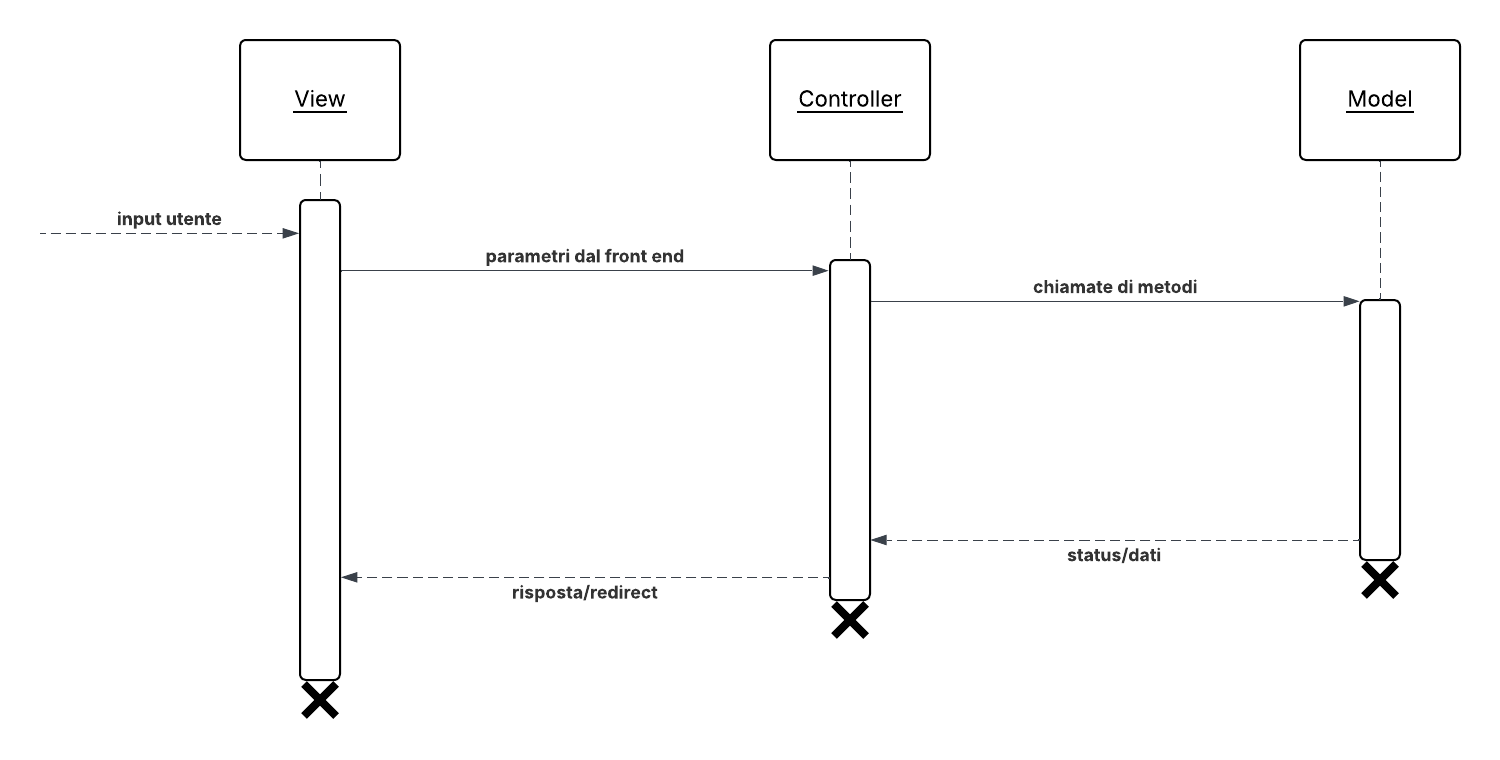
\includegraphics[width=0.8\linewidth]{Sequence Diagram pattern MVC.png}
\caption{Sequence diagram che illustra il flusso di interazione nel pattern MVC}
\label{fig:mvc-sequence}
\end{figure}
Infine nella root directory del progetto si trovano i file di supporto come il README.md inizializzato nel momento in cui è stata creata la repository gestita tramite
\textit{Gitflow}\cite{gitflow}, il CHANGELOG.md che serve a tenere presente le versioni dei rilasci 
e il Gemfile.rb che consiste nella lista delle gemme di Ruby aggiunte nel progetto ossia le librerie aggiuntive scaricate nel progetto.
Nel caso di questo software il client è stato sostituito con un client scritto in ReactJS e quindi di Ruby On Rails vengono usate principalmente le componenti
per costruire il server mentre le Views vengono utilizzate per definire template interni come le e-mails.
\par L'\textit{ActiveRecord} è la componente del framework di Rails che gestisce l'accesso al database e fornisce un'interfaccia object-oriented per interagire con le tabelle
del database MySQL. In particolare implementa il pattern \textit{Create-Read-Update-Delete} (CRUD)\cite{ibm_crud} che permette di creare, visualizzare, modificare
o cancellare record. Queste operazioni sono implementate direttamente nel codice senza la necessità di dover scrivere SQL puro. Ad esempio, ogni classe ha un metodo built-in dinamico
chiamato .create() a cui vengono passati in formato chiave-valore i parametri corrispondenti agli attributi del modello dati e sarà il linguaggio stesso a tradurre
quel codice in SQL puro da eseguire sul database collegato al progetto. È molto vantaggioso dal punto di vista della semplicità e leggibilità del codice dato che
non essendo necessario scrivere SQL puro che poterbbe risultare molto difficile da capire.
Reperire l'informazione dal database è un'operazione fondamentale del software e come sappiamo viene eseguita attraverso query che possono essere anche molto intricate
da scrivere e da comprendere. L'ActiveRecord semplifica questa operazione permettendo di scrivere clausole WHERE attraverso il metodo .where() che identifica la classe dell'oggetto
a cui è applicato e i parametri passati allo stesso modo di come vengono passati alla creazione seleziona i record interessati. Esiste anche un metodo .select\{\} che però va utilizzato
attraverso la classe di oggetti Proc in uno stile funzionale rielaborato nel linguaggio Ruby, si noti l'utilizzo di parentesi graffe al posto di quelle tonde. Spesso nei linguaggi
object-oriented più vecchi iterare attraverso una lista di oggetti si rivelava un'operazione che necessitava di molte risorse e richiedevano una gestione manuale dell'indicizzazione di essi.
Ovviamente con l'introduzione di nuove tecnologie moderne il problema si è risolto attraverso costrutti come gli iteratori ma verso la fine degli anni Novanta quando Ruby era in sviluppo
questi non erano ancora stati introdotti. Però esisteva già il paradigma funzionale che non prevedeva la presenza di oggetti e operava solo attraverso funzioni e dati semplici.
I linguaggi funzionali sono conosciuti principalmente per la sintassi molto diversa da quella dei linguaggi object-oriented e per la loro particolare affinità alla gestione
efficiente delle liste di dati attraverso funzioni come map che applica una funzione ad ogni elemento della lista, filter per filtrare i dati che rispettano una certa condizione booleana,
le lambda per implementare le funzioni anonime e molte altre.
e molte altre. Lo sviluppatore di Ruby ha pensato di introdurre la possibilità di iterare attraverso una lista in stile funzionale ma mantenendo l'approccio object-oriented.
In Ruby le funzioni applicate in questo modo si chiamano "blocchi" e si appoggiano alla classe Proc, quindi anche le funzioni sono oggetti e hanno i loro metodi definiti.
Per cui l'operazione di SELECT si può condensare con la clausola WHERE attraverso il metodo .select\{\} in cui verrà definita una condizione come viene fatto nel metodo .where() e verranno
selezionati solo i record che la rispettano. Il vantaggio del metodo .select\{\} è che si può applicare anche a liste di strutture diverse da oggetti dell'ActiveRecord.
L'operazione di UPDATE viene eseguita attraverso il metodo .update() con i parametri passati come nel caso del metodo .create().
Infine l'ultima operazione di DELETE a disposizione viene implementata dal metodo .destroy che elimina dal database il record a cui è applicato.
\par Per quanto riguarda la gestione delle richieste effettuate secondo il protocollo HTTP essa è affidata ad un file routes.rb in cui si scrivono i percorsi agli endpoints del sito.
Una route viene definita accostando il verb del tipo di richiesta che si intende implementare quindi se è una GET, POST, PUT, DELETE o PATCH, il percorso nel progetto per arrivare al
file che contiene il metodo che rappresenta l'endpoint e una clausola to: nome\_classe\#nome\_endpoint. Il modulo prevede che la sezione principale di ricerca sia disponibile in una sezione a
cui un utente autenticato possa liberamente utilizzare e la stessa pagina disponibile in area pubblica dove utenti non autenticati possano provare ad utilizzare la funzionalità.
Il framework Rails permette di utilizzare lo stesso endpoint e collegarlo a due punti diversi del sito web, una copia del percorso all'endpoint si troverà sotto una keyword "unauth"
e l'altra sarà nella sezione ordinaria. La classe built-in per eseguire le richieste HTTP è \textit{Net::HTTP} che non richiede alcun servizio aggiuntivo e può essere usata facilmente
in un'applicazione sviluppata con Rails. Una richiesta ad un'API integrata nel software tramite API Key e Bearer Token per esempio viene inizialmente creata come un nuovo oggetto poi
vengono passati come parametro un URI (Uniform Resource Identifier) che identifica l'endpoint esterno a cui inviare la richiesta e il body in forma di oggetto con attributi chiave-valore
in forma di stringa o di JSON aggiungendo eventuali parametri opzionali come opzioni di timeout o altri token di autenticazione. Questo comando si può salvare in una variabile che
assumerà il valore della risposta del server esterno. Tuttavia nel progetto è preferito il servizio opern-source offerto con la gemma \textit{Faraday}\cite{faraday_gem} che aiuta a separare
la logica di composizione e autenticazione delle richieste da quella del software vero e proprio. In questo modo permette di scegliere un adapter per effettuare le richieste, che può essere
Net::HTTP stesso, implementando un'interfaccia astratta comune a tutte le richieste API dirette verso l'esterno. Faraday inoltre permette di manipolare direttamente alcuni aspetti delle richieste
come i formati dei body di richiesta e risposta, i retry in caso di fallimento, la gestione delle credenziali di autenticazione e le modalità di lancio delle eccezioni. Faraday viene
preferito perchè utilizare Net::HTTP nel codice lo rende più verboso dato che serve gestire le eccezioni direttamente dove viene fatta la chiamata quindi non è un buon approccio per
quanto riguarda la leggibilità e mantenibilità di esso. Allora una nuova interfaccia da implementare erediterà i metodi dell'interfaccia generica di Faraday e dipenderà esclusivamente da
quest'ultima. Le uniche cose da implementare sono i singoli metodi che rappresentano i tipi di richiesta da effettuare verso l'esterno, ma qualsiasi richiesta HTTP passerà per l'interfaccia
astratta di Faraday.

\subsection{Gitflow}

\subsection{Amazon Web Services}
Come anticipato prima, il blocco di servizi offerti da Amazon Web Services sono una componente molto importante dei software sviluppati in azienda.
AWS è una piattaforma di cloud computing che dispone di un catalogo di oltre 200 servizi IT on-demand accessibili via Internet con un modello di pagamento a consumo. Per questo software l'archiettura 
è stata realizzata attraverso \textit{Elastic Compute Cloud} (EC2) che permette di definire più istanze della stessa applicazione per far funzionare i tre ambienti del sito:
development ossia l'ambiente di sviluppo, staging che è l'ambiente in cui vengono rilasciati gli incrementi del software in modo che il cliente li possa testare
e production che è l'ambiente su cui funziona il sito ufficiale e che viene utilizzato dai clienti. L'accesso ai diversi server è gestito tramite \textit{Secure Shell Protocol}\cite{rfc4251} (SSH)
A livello di repository ogni istanza utilizza il codice dei branch omonimi e questo viene gestito attraverso \textit{CodePipeline}, un altro servizio di AWS che gestisce le fasi
di rilascio con uno script in Python e il servizio di containering di \textit{Docker}\cite{docker}. Questi containers sono monitorati dal servizio di \textit{Cloudwatch} che
registra i log di ogni container, utili per le sessioni di debugging. Anche i database sono separati e istanziati attraverso il servizio \textit{Aurora and RDS} in modo che ogni
ambiente abbia il suo storage. Allo stesso modo di EC2, RDS permette di creare delle istanze alle quali si può accedere singolarmente tramite SSH per ogni database \textit{MYSQL}\cite{mysql}.
\textit{S3} è un servizio di storage in cloud che dà la possibilità di salvare media di qualsiasi tipo utilizzati nel software. Risulta particolarmente utile perchè permette di separare
la componente miscellanea dal software riducendone la dimensione effettiva. Si utilizza creando dei bucket che non sono niente meno di directory a cui ci si può collegare
da remoto e caricare, cancellare, aggiornare i media necessari. Infine viene utilizzato il servizio \textit{DynamoDB} che offre un database NoSQL serverless,
utile per immagazzinare dati non strutturati, nel caso di questo software si parla delle notifiche utilizzate per gestire il sistema di notifiche che segnalano lo stato di
avanzamento e conclusione dei processi asincroni ampliamente utilizzati nello sviluppo di questo modulo.
Nel software è implementata anche una interfaccia che si connette al servizio Cognito che trova la sua utilità nella validazione del login di un utente nel momento in cui il back end
riceve il token JWT dal front end (il flusso di autenticazione dell'utente è descritto nelle sezioni successive).
Le email sono inviate attraverso il servizio Simple Email Service (SES) 
% Aggiungere Cognito e Ses
\subsection{Sidekiq}

I processi asincroni che d'ora in avanti saranno chiamati "job" sono gestiti attraverso una gemma di Ruby On Rails che si appoggia a \textit{Redis}\cite{redis_home} (REmote DIctionary Server), un
data store open source che può essere utilizzato come database, cache o broker di messaggi. Funziona salvando i dati nella RAM in forma di chiave-valore minimizzando le latenze nell'ordine dei microsecondi
dato che l'accesso ai dati salvati su disco è più lento rispetto all'accesso dei dati presenti in RAM. In questo caso Redis viene utilizzato per salvare le informazioni necessarie ai
job per svolgere le loro computazioni, di conseguenza ottimizza la velocità di esecuzione del job dato che l'accesso ai dati è molto veloce.
I vengono creati attraverso la gemma di Ruby On Rails di \textit{Sidekiq}\cite{sidekiq} che mette a disposizione un efficiente sistema di gestione di processi asincroni attraverso
metodi di una superclasse da sfruttare attraverso l'ereditarietà delle classi che implementano questo tipo di asincronismo. Il job viene astratto come un oggetto, dopotutto in
Ruby qualsiasi entità è un oggetto, con i suoi attributi fra cui i più rilevanti sono lo status, la data di creazione, di inzio e di fine processo e l'identificativo dell'oggetto che
implementa asincronismo. Il ciclo di vita è molto semplice: alla creazione ha status "running" e alla risoluzione diventa "complete" mentre se occorrono eccezioni durante la sua esecuzione
si imposta automaticamente uno status "error" e salva il messaggio d'errore in un campo apposito. La classe che implementa questo meccanismo deve possedere obbligatoriamente un metodo
"resolve\_job" che si potrà chiamare da qualsiasi punto del codice su un'istanza dell'oggetto e che svolgerà il suo task per poi concludere ed impostare lo stato "complete" aggiornando
anche il timestamp di fine. Spesso il front end avrà bisogno di ricevere un segnale che un certo processo ha concluso il suo task e l'esito finale di esso.
A questo scopo si usa un sistema di notifiche in tempo reale che comunichi lo stato finale del job ed eventualmente apportando dei dati che al front end in modo che quest'ultimo sappia
se poter proseguire con un redirect ad un'altra pagina mostrare un messaggio d'errore. Queste notifiche vengono salvate sul database di DynamoDB, servizio di AWS citato
prima e vengono cancellate dopo un dato periodo di tempo che sono state utilizzate. Questo sistema di asincronismo contribuisce al parallelismo di task uguali tra loro rendendo
l'applicazione più responsiva e migliorando le prestazioni. Con Sidekiq vengono gestiti due tipi di job: i job ordinari e i cron job. I primi vengono definiti ognuno nel suo file nella directory
/sidekiq e per essere eseguiti devono essere eseguiti nel codice. La funzionalità richiesta in questo modulo però aveva la necessità di eseguire job senza doverli implementare nel codice che quindi
venissero messi in coda ed eseguiti periodicamente e autonomamente dall'applicazione. Questo requisito viene soddisfatto con il supporto della gemma \textit{sidekiq-cron}\cite{sidekiq_cron_gem} che
permette di creare un file con estensione .yml che agisca da scehduler. Creato il file del job la sua esecuzione si può automatizzare scrivendo nello scheduler delle stringhe come '0 5 * * *' (questa forma
significa "esegui il job ogni giorno alle ore 5") accostando il nome della classe del job in modo che sappia quale file eseguire.

\section{I servizi esterni}

\subsection{Stripe}

Per la gestione del processo di pagamento, con particolare attenzione alle modalità di addebito ricorrente caratteristiche di un sistema di abbonamenti,
è stato integrato il servizio di \textit{Stripe}\cite{stripe} attraverso la gemma ufficiale per Ruby\cite{stripe_ruby_gem}. Il servizio offre un sistema di gestione dei pagamenti
basato su oggetti ed utilizzabile attraverso diversi linguaggi di programmazione oltre a Ruby fra cui Python, Java, .NET e altri. Si integra
bene con Ruby per il fatto che anche l'API di Stripe opera via oggetti identificati univocamente da object id e ha classi di oggetti con i loro attributi e metodi quindi allineandosi
perfettamente con il paradigma object oriented.
Offre molte classi per implementare flussi di pagamento e le più rilevanti nello sviluppo di questo modulo sono per esempio le classi Payment Intents, Subscriptions, Payment Methods,
Invoices, Tax Rate, Customers e tante altre che verranno illustrate approfonditamente assieme al flusso della funzionalità nel prossimo capitolo.
Stripe si è rilvelata una scelta vantaggiosa anche per il fatto che la gestione dei dati sensibili non è delegata al back end dell'applicazione ed è interamente
a carico del servizio stesso. Un altro punto di forza di questa API è la documentazione chiara\cite{stripe_api_reference} e la disponibilità di assistenza 24 ore su 24 da parte
del team di supporto di cui il team si è potuto avvalere per far fronte alle difficoltà incontrate durante il lavoro ad alcuni task.

\subsection{RabbitMQ}

L'analisi dei domini è stata affidata al servizio di \textit{RabbitMQ}\cite{rabbitmq}, un middleware message-oriented che implementa il protocollo \textit{Advanced Message Queuing Protocol}
(AMPQ) per gestire le richieste in entrata dall'applicazione e restituire in risposta gli stessi dati rielaborati.
L'integrazione avviene attraverso un server lato servizio che riceve le richieste in formato JSON ricevute attraverso un canale che collega tale server e l'applicazione.
La comunicazione viene aperta dopo l'autenticazione avvenuta con successo tramite nome utente e password.
Il servizio opera principalmente secondo il pattern publish/subscribe. In pratica l'applicazione pubblica su una coda i dati interessati che devono essere elaborati,
poi questo dato pubblicato viene prelevato ed elaborato, tecnicamente "consumato", dal server lato servizio che a fine elaborazione viene ripubblicato su una coda diversa
a cui l'applicazione si sottoscrive periodicamente per ricevere la risposta con i dati rielaborati.
Questo tipo di comunicazione non passa per l'interfaccia di Faraday citata nelle sezioni precedenti poichè non sono richieste HTTP.

\subsection{Gemme di Ruby}

In un progetto così grande viene utilizzato un discreto numero di gemme, alcune utilizzate in tutti gli ambienti, altre solo in ambiente
di sviluppo che agevolano gli sviluppatori nell'attività di implementazione del codice.
\textit{ActiveModelSerializers}\cite{active_model_serializers_gem} è una gemma che viene impiegata all'interno del progetto per modificare a proprio
piacimento le risposte tornate dagli endpoint del back end al front end. Le risposte di base sono in JSON ma non sono ben strutturate, tendono a tornare un oggetto
contenente attributi chiave-valore semplici. Questo strumento permette tuttavia di allineare il contenuto della risposta alla classe dell'oggetto tornato aggiungendo
nella risposta gli attributi di esso presenti nel suo record a database. Inoltre si possono anche creare attributi chiave-valore personalizzati derivati da altri
attributi dato che nel modulo si possono definire funzioni oppure si può fare presente al modulo che l'oggetto preso in esame ha un attributo foreign key di un
oggetto di una classe diversa e quindi nella risposta sarà presente come oggetto annidato anche il record dell'oggetto collegato.
\par Nel progetto è importante definire i livelli di accesso alle pagine fra utenti con permessi diversi. Ad esempio, un utente con ruolo superadmin può accedere
più o meno a tutte le pagine del sito dato che funge da amministratore della piattaforma. Un utente base invece sarà abilitato ad accedere alcune sezioni a cui
un superadmin può liberamente accedere. Questo aspetto viene gestito tramite una combinazione di \textit{CanCanCan}\cite{cancancan_gem} utilizzato per implementare
il modello \textit{Role Based Access Control} (RBAC)\cite{ibm_rbac} e la gemma \textit{json-jwt}\cite{json_jwt_gem} per la validazione del JSON Web Token (JWT) che
certifica l'identità dell'utente. RBAC è un modello di autorizzazione dell'utente di accesso alle risorse in cui un amministratore assegna ad ogni utente uno i pìu ruoli.
CanCanCan permtte di implemetare questo modello definendo delle classi custom in una directory "abilities" nominate a seconda del ruolo che si intende codificare
in cui si possono scrivere delle istruzioni composte da "can" oppure "cannot", nome dell'endpoint a cui si vuole dare o meno l'accesso, classe dell'oggetto in cui
l'endpoint è definito ed eventuali parametri come l'identificativo dell'utente se si vuole fare in modo che nessun altro utente a parte l'amministratore possa accedere
ad una certa risorsa. 
% Da rivedere il flusso di login
Il JWT valida l'identità dell'utente al momento del login con le credenziali da parte dell'utente. Il front end raccoglie i dati di accesso e
alcune informazioni rilevanti in un oggetto che poi viene crittato con un algoritmo di crittazione e firmato digitalmente, RSA in questo caso, e inviato al back end
che attraverso una richiesta API ad \textit{AWS Cognito} verifica se i dati di accesso sono corretti e restituire le informazioni sull'utente in risposta.
\par A supporto dello sviluppo in ambiente di test vengono utilizzate le gemme del framework di testing per Ruby, \textit{RSpec}\cite{rspec_home} che verrà spiegato
approfonditamente nel capitolo riguardante il testing del modulo. Nella test suite del progetto vengono utilizzate anche le gemme \textit{faker}\cite{faker_gem}
che permette di creare facilmente dati finti ma ben strutturati che rendono i test molto più realistici e \textit{webmock} che permette di creare dei moduli utili
alla scrittura di stub. Questi ultimi sono necessari per far funzionare i test delle richieste API verso servizi esterni dato che quelle reali sono disabilitate
dal framework di RSpec quindi vengono scritte delle risposte hard-coded in file JSON che contribuiscono a simulare internamente l'interazione con l'esterno.
Scrivendo in questo modo le risposte però si perde la variabilità dei dati nel senso che due risposte ricevute dallo stesso endpoint dell'API potrebbero essere
elaborate nell'applicazione in modo differente a seconda di un flag e se il file hard-coded è scritto con un valore per il flag, si potrà effettuare il test del
comportamento del software solo nel caso in cui ci sia quel valore. Si può andare a cambiare manualmente il valore nel file ma non sarebbe un approccio efficiente
poichè si punta all'automatizzazione completa dei test. Il problema viene risolto attraverso la gemma \textit{factory\_bot\_rails}\cite{factory_bot_rails_gem} che
si rivela fondamentale nella scrittura dei test. Essa permette la creazione rapida di oggetti finti in un database di test gestito con SQLite
che viene cancellato e ricreato ogni volta che si avviano i test automatici. Oggetti e strutture hanno dati fissi che si possono comunque alterare in blocchi
before i cui comandi vengono eseguiti prima di eseguire il test effettivo ma per evitare di fare questa cosa per ogni singolo test case con factory\_bot si possono
definire dei trait in cui si possono definire le alterazioni più comuni. Ad esempio, se il modello dati che rappresenta l'utente ha un attributo "role" per il ruolo
dell'utente nella piattaforma e il valore di default è "user" ma serve un utente "admin" in più test diversi, si può definire un trait "admin" che quando viene chiamato
alla creazione di un utente finto questo verrà istanziato con il ruolo desiderato. Lo stesso vale anche per le richieste API che hanno dei valori di default che si
possono alterare con dei trait e rendere i test case completi. Dalla definizione degli integration test la gemma \textit{Rswag}\cite{rswag_gem} trae le informazioni
necessarie alla generazione di un file con estensione .yml che codifica uno swagger che funge da documentazione API automatica utile al front end per capire come
strutturare alcune richieste al back end.
\par È risaputo che è molto complicato realizzare un software completamente a prova di errori, per quanto si provi a gestirli e ad evitarle che si verifichino, in qualche
modo le eccezioni possono verificarsi in qualsiasi momento. Lo strumento utilizzato in azienda per catturare le eccezioni è \textit{Sentry}\cite{sentry}, letteralmente "sentinella".
L'applicazione integra questo servizio attraverso le gemme \textit{sentry-rails}\cite{sentry_rails_gem} e \textit{sentry-sidekiq}\cite{sentry_sidekiq_gem}, la prima
sorveglia l'applicazione principale mentre l'altra monitora le eccezioni derivanti dai job asincroni creati tramite Sidekiq.
Sentry ha il suo file di configurazione all'interno dell'applicazione quindi automaticamente rileva le eccezioni ma in alcuni punti del codice potrebbe essere necessario
formattare un errore più preciso in modo che venga rilevato con un messaggio d'errore deciso dallo sviluppatore.
Sul sito web del servizio ci sono alcune funzionalità di monitoring ma quella che viene utilizzata è principalmente la lista degli errori rilevati e il report
settimanale con il resoconto delle transazioni e degli errori rilevati nel software. Degli errori catturati Sentry mostra il messaggio d'errore con una descrizione,
il numero di occorrenze nel periodo di tempo per cui è impostato il filtro, il linguaggio di programmazione e il sistema operativo rilevati, l'ambiente in cui si è
verificati, se arriva da Sidekiq oppure dall'applicazione, una sezione che mostra il codice critico, tutta la trace quindi il percorso fatto per arrivare all'errore
dall'inizio al codice critico, le query eseguite e alla fine una sezione con elenchi di dati che riassume le informazioni generali dell'errore come l'url della richiesta
e i parametri inviati. Avere una schematizzazazione delle eccezioni spesso risulta in un buon supporto all'attività di debugging senza la quale potrebbe rivelarsi molto
complicato risalire al punto esatto in cui si è verificato l'errore. Un altro punto di forza di questo servizio è che si può integrare con Slack in modo da avere un canale per progetto che
notifica il fatto che sia stato rilevato un errore con un messaggio che contiene il collegamento alla pagina che raccoglie le informazioni su di esso.
\par I servizi di AWS pervadono profondamente il progetto dall'architettura, fino alle funzionalità. Vengono utilizzate delle gemme per il Software Development Kit (SDK)
per AWS\cite{aws_sdk_ruby} in Ruby come nel caso di S3, Dynamo e Cognito. Queste gemme semplificano l'utilizzo dei servizi di AWS fornendo delle librerie che
nel progetto sono risultate particolarmente utili per la realizzazione dei moduli senza i quali l'applicazione non potrebbe collegarsi ai server di Amazon.
Integrando le gemme di AWS specifiche per Ruby si ha a disposizione un macro-modulo omonimo che contiene le sottoclassi che implementano una serie di altre sottoclassi e
metodi che sarebbero molto complessi da definire senza questo prezioso strumento di supporto.
\par Ultima gemma ma non per importanza c'è \textit{Awesome Print}\cite{awesome_print_gem}. Sviluppando software in Ruby la funzione più utilizzata è probabilmente quella di print che
stampa a terminale il valore degli oggetti o variabili passate. Le funzioni built-in di stampa in Ruby sono:
\begin{itemize}
    \item puts: put string, stampa il parametro passato applicando il metodo .to\_s (to string) e aggiungendo un carattere \textbackslash n (new line) alla fine;
    \item print: esegue la stessa operazione eseguita da puts ma senza aggiungere il carattere \textbackslash n;
    \item p: stampa le strutture in modo completo, ad esempio se si vuole stampare una variabile che rappresenta un array verranno stampate anche le parentesi
          quadre che con puts non si vedrebbero, utile per gli sviluppatori;
    \item pp: pretty print, utile per visualizzare strutture dati complesse come hash innestati;
    \item print/sprintf: formattano l'output attraverso stringhe di formato, ad esempio "\%d", allo stesso modo di come si scrive in C.
          La seconda applica anche il metodo .to\_s dopo aver formattato e composto la stringa.
\end{itemize}
Nonostante la presenza di tutte queste funzioni, nessuna di esse stampa in un formato intuitivo gli oggetti gestiti dall'ActiveRecord quindi la rappresentazione
visiva dei record nel database non è il massimo se si prova a stamparne uno con le fuzioni citate sopra. Awesome Print implementa un metodo globale ap nella classe Object che
è la classe padre di quasi tutte le altre classi di Ruby. Il metodo si può utilizzare in tutti i file con estensione rb contenenti codice eseguibile in cui abbia senso utilizzarlo
dato che nel file delle routes oppure nei file di configurazione del progetto non avrebbe significato.
Stampando un record tramite il metodo ap l'output sarà più colorato ed indentato per livelli di profondità in modo che sia facilmente leggibile e distinguibile dal resto
dell'output sul terminale che di default è bianco su nero. ap non è ristretto agli oggetti della classe ActiveRecord ma si può applicare anche a qualsiasi variabile o costante.
Stampando una stringa questa verrà colorat di giallo nell'output, i numeri interi saranno blu mentre quelli decimali appariranno rosa sul temrinale.
Sembra un cosa da poco ma nelle attività di debugging aiuta a visualizzare ed identificare con un'occhiata strutture che se fossero colorate di bianco e formattate male
risulterebbero molto complesse da analizzare, sprecando anche tempo nel peggiore dei casi.


\begin{figure}[h]
\centering
\includegraphics[width=1\linewidth]{Deployment Diagram.png}
\caption{Deployment diagram che mostra le interazioni fra i servizi utilizzati}
\label{fig:dep_diagram}
\end{figure}

\chapter{Funzionalità Sviluppata}

% Sistema o funzionalità sviluppata: casi d'uso, deployment diagram, comportamentale tipo activity
Il software essendo un e-commerce ha un flusso di utilizzo da parte di un utente generico molto semplice: cercare il prodotto desiderato,
aggiungerlo al carrello in caso lo si voglia acquistare, effettuare il pagamento e il check-out ed infine usufruire del prodotto acquistato.
% Spiegazione realizzazione delle email
Queste ultime sono dinamiche poichè quando viene utilizzata una funzione che ne invia una o più vengono passati dei parametri al template, altrimenti non si
potrebbe cambiare il nome dell'utente destinatario. Ma se le views non sono collegate ad un controller come succede nell'utilizzo canonico di Ruby On Rails, allora
non avrebbero modo di ricevere parametri. Il problema viene risolto facilmente attraverso una combinazione di OpenStruct e \textit{GraphQL}.
La prima è una classe built-in della libreria standard di Ruby

\chapter{Valutazione}

Valutazione con testing in RSpec (https://github.com/simplecov-ruby/simplecov), questionario sul software per valutare
la bontà del prodotto e la soddisfazione degli utenti (va bene anche il team sviluppatori) -> da fare ad es su google forms o
microsoft forms con likert e domanda aperta per raccogliere feedback

\chapter{Conclusioni e Sviluppi Futuri}

conclusioni e sviluppi futuri


%% Fine dei capitoli normali, inizio dei capitoli-appendice (opzionali)
\appendix

%\part{Appendici}

% \chapter{Titolo della prima appendice}
% Sed purus libero, vestibulum ut nibh vitae, mollis ultricies augue. Pellentesque velit libero, tempor sed pulvinar non, fermentum eu leo. Duis posuere eleifend nulla eget sagittis. Nam laoreet accumsan rutrum. Interdum et malesuada fames ac ante ipsum primis in faucibus. Curabitur eget libero quis leo porttitor vehicula eget nec odio. Proin euismod interdum ligula non ultricies. Maecenas sit amet accumsan sapien.

%% Parte conclusiva del documento; tipicamente per riassunto, bibliografia e/o indice analitico.
\backmatter

%% Riassunto (opzionale)
%\summary
%Maecenas tempor elit sed arcu commodo, dapibus sagittis leo egestas. Praesent at ultrices urna. Integer et nibh in augue mollis facilisis sit amet eget magna. Fusce at porttitor sapien. Phasellus imperdiet, felis et molestie vulputate, mauris sapien tincidunt justo, in lacinia velit nisi nec ipsum. Duis elementum pharetra lorem, ut pellentesque nulla congue et. Sed eu venenatis tellus, pharetra cursus felis. Sed et luctus nunc. Aenean commodo, neque a aliquam bibendum, mauris augue fringilla justo, et scelerisque odio mi sit amet diam. Nulla at placerat nibh, nec rutrum urna. Donec ut egestas magna. Aliquam erat volutpat. Phasellus vestibulum justo sed purus mattis, vitae lacinia magna viverra. Nulla rutrum diam dui, vel semper mi mattis ac. Vestibulum ante ipsum primis in faucibus orci luctus et ultrices posuere cubilia Curae; Donec id vestibulum lectus, eget tristique est.

%% Bibliografia (praticamente obbligatoria)
\bibliographystyle{plain_\languagename}%% Carica l'omonimo file .bst, dove \languagename � la lingua attiva.
%% Nel caso in cui si usi un file .bib (consigliato)
\bibliography{thud}
%% Nel caso di bibliografia manuale, usare l'environment thebibliography.

%% Per l'indice analitico, usare il pacchetto makeidx (o analogo).

\end{document}
